%------------------------------------------------
\section{Тяжелоионная мода}
%------------------------------------------------

\begin{frame}
	\frametitle{Время жизни пучка}
	
\begin{columns}[t]
	\begin{column}{0.5\textwidth}
\par Временная эволюция эмиттанса и разброса импульса при наличии процессов охлаждения

\small \begin{equation}
\begin{aligned}
& \dv{\varepsilon}{t}=\underbrace{-\frac{1}{\tau_{\text{tr}}} \cdot \varepsilon}_{\text {cooling}}+\underbrace{\left(\dv{\varepsilon}{t}\right)_{\text{IBS}}}_{\text{heating}} \\
& \dv{\delta^2}{t}=\underbrace{-\frac{1}{\tau_{\text{long}}} \cdot \delta^2}_{\text {cooling}}+\underbrace{\left(\dv{\delta^2}{t}\right)_{\text {IBS}}}_{\text {heating}} \\
&
\end{aligned}
\end{equation} \normalsize 	
	 \end{column}
	 \begin{column}{0.5\textwidth}
	 \par Темп охлаждения в отсутствии шума
	  	\small \begin{equation}
	 	\frac{1}{\tau_{\text{tr}}}=\frac{W}{N}\frac{\left(1-1/{M_{\text{pk}}}^2\right)^2}{M_{\text{kp}}}
	 	\end{equation} \normalsize 
	\par Коэффициент перемешивания (mixing factors)
	\par Пикап-киккер, киккер-пикап
	  	\small \begin{equation}
		\begin{aligned}
		M_{\text{pk}}&=\frac{1}{2\left(f_{\text{max}}+f_{\text{min}}\right)\eta_{\text{pk}}T_{\text{pk}}\delta} \\
		M_{\text{kp}}&=\frac{1}{2\left(f_{\text{max}}-f_{\text{min}}\right)\eta_{\text{kp}}T_{\text{kp}}\delta}
		\end{aligned}
	 	\end{equation} \normalsize 
          \end{column}
\end{columns}

\end{frame}

%------------------------------------------------
\begin{frame}
	\frametitle{Комбинированная структура}
\begin{columns}[t]
        \begin{column}{0.5\textwidth}
\par В случае “комбинированной” структуры одна арка регулярная, в то время как другая использует резонансную модуляцию.

\small \begin{equation}        
\eta_{\text{pk}}=1/\gamma_{\text{tr}}^2-1/\gamma^2
\end{equation} \normalsize 
\small \begin{equation}        
\eta_{\text{kp}}=-1/\gamma_{\text{tr}}^2-1/\gamma^2
\end{equation} \normalsize 

\par Резонансную арку можно получить из регулярной, введя дополнительное семейство фокусирующих квадруполей.

        \end{column}
        \begin{column}{0.5\textwidth}
            \begin{figure}[t]
                \centering
                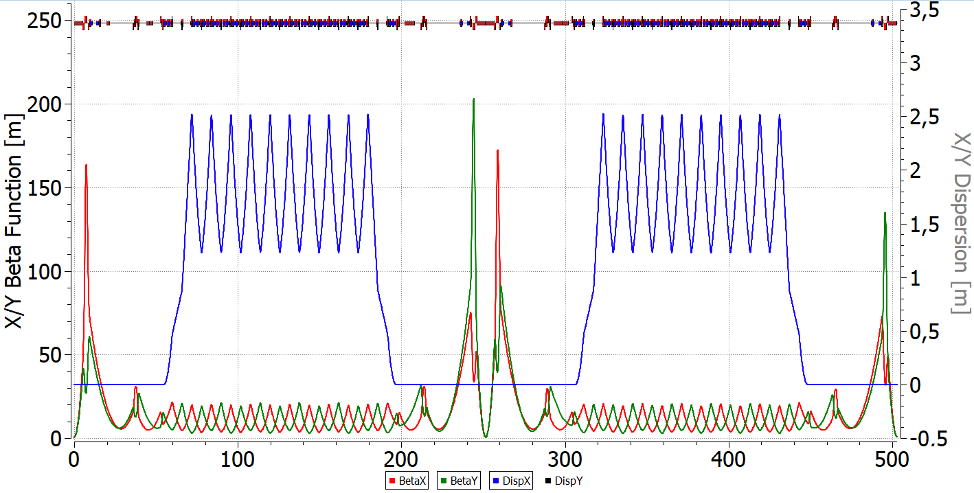
\includegraphics[width=6cm]{regular}
                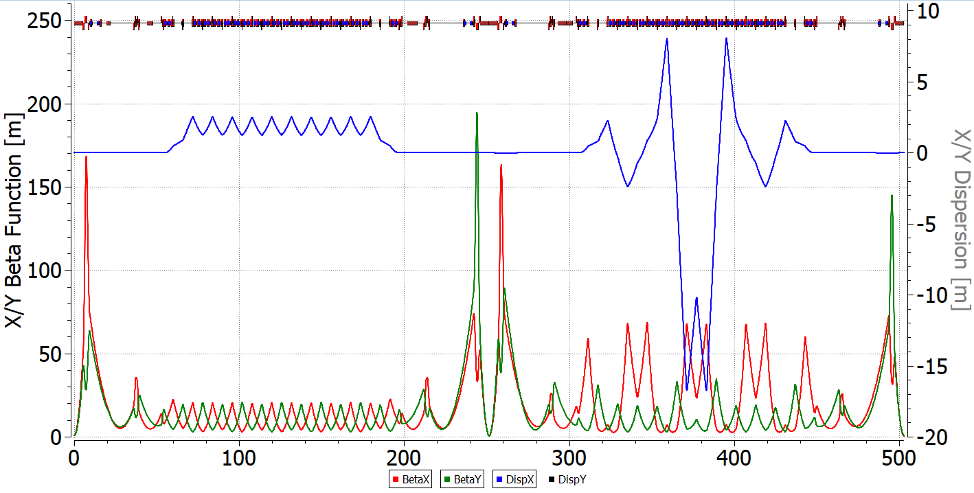
\includegraphics[width=6cm]{combined}
                \label{fig:structures}
            \end{figure}
        \end{column}
    \end{columns}
\end{frame}

%------------------------------------------------
\begin{frame}
	\frametitle{Стохастическое охлаждение}
	\begin{figure}[h!]
		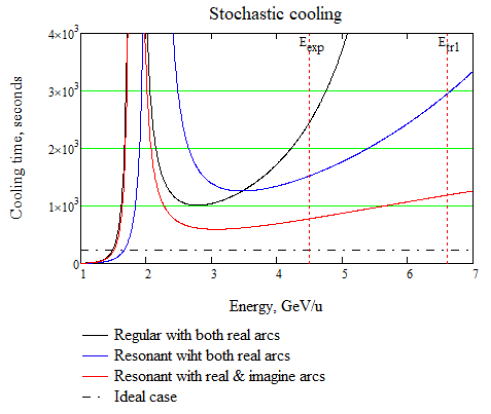
\includegraphics[width=6cm]{images/SC}
		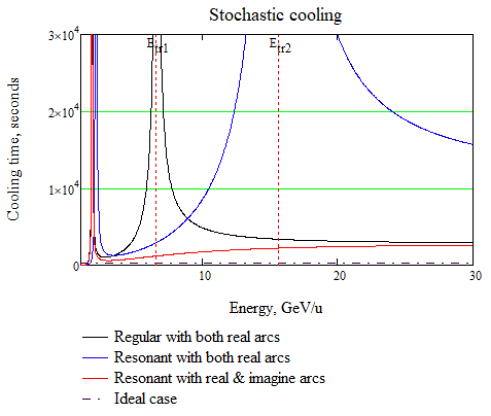
\includegraphics[width=6cm]{images/SC_wide}
                \label{Figure 1}
	\end{figure}
\end{frame}


%------------------------------------------------
\begin{frame}
	\frametitle{Внутрипучковое рассеяние}
\begin{center}
Темп внутрипучкового рассеяния	
\end{center}

\small \begin{equation}
\frac{1}{\tau_{\text{IBS}}}=\frac{\sqrt{\pi}}{4} \frac{c Z^2 r_p^2 L_{\text{C}}}{A} \cdot \frac{N}{C_{\text{orb}}} \cdot \frac{\left\langle\beta_x\right\rangle}{\beta^3 \gamma^3 \varepsilon_x^{5 / 2}\left\langle\sqrt{\beta_x}\right\rangle}\left(\left\langle\frac{D_x^2+\dot{D}_x^2}{\beta_x^2}\right\rangle-\frac{1}{\gamma^2}\right)
\end{equation} \normalsize

            \begin{figure}[h!]
                \centering
                % \caption{Hawkins et al, 2015}
                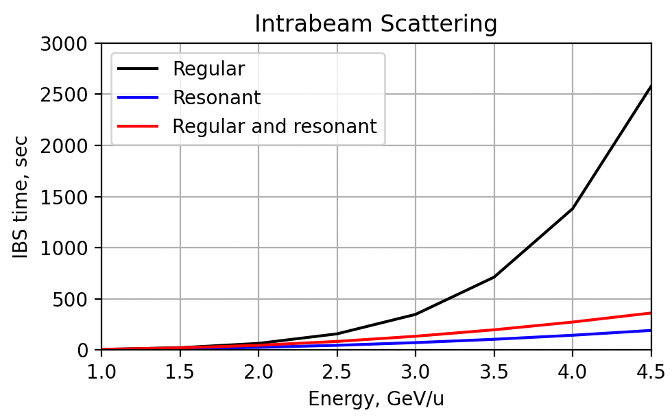
\includegraphics[width=6cm]{images/IBS}
                \label{fig:ibs}
            \end{figure}
	
\end{frame}